\documentclass[nohyper,nobib]{tufte-book} % Vergeet bij uitprinten niet te switchen naar a4paper optie
\usepackage{cleveref} %hyperref werkt niet in deze klasse
\usepackage{nameref}
\usepackage[dutch]{babel}
\usepackage{csquotes}
\usepackage{microtype}
\usepackage{tikz}
\tikzset{>=latex}
\usetikzlibrary{positioning,calc,decorations.pathreplacing}
\usepackage{graphicx}
\usepackage{array,booktabs,multirow}
\usepackage[backend=biber, natbib=true, style=numeric]{biblatex}
\addbibresource{bib.bib}
\newcommand{\afdelingj}{afdeling~J }
\newcommand{\Afdelingj}{Afdeling~J }
\usepackage{epigraph}
%% Metadata book
\title{Oriënterend Zorgstage}
\author{Edon Namani}
\date{\today}
\publisher{Naam\sidenote{\texttt{dummymail@mail.com}}}

%%%% Kevin Godny's code for title page and contents from https://groups.google.com/forum/#!topic/tufte-latex/ujdzrktC1BQ
\makeatletter
\renewcommand{\maketitlepage}{%
\begingroup%
\setlength{\parindent}{0pt}

{\fontsize{24}{24}\selectfont\textit{\@author}\par}

\vspace{1.75in}{\fontsize{36}{54}\selectfont\@title\par}

\vspace{0.5in}{\fontsize{14}{14}\selectfont\textsf{\smallcaps{\@date}}\par}

\vfill{\fontsize{14}{14}\selectfont\textit{\@publisher}\par}

\thispagestyle{empty}
\endgroup
}
\makeatother

\titlecontents{part}%
    [0pt]% distance from left margin
    {\addvspace{0.25\baselineskip}}% above (global formatting of entry)
    {\allcaps{Deel~\thecontentslabel}\allcaps}% before w/ label (label = ``Part I'')
    {\allcaps{Deel~\thecontentslabel}\allcaps}% before w/o label
    {}% filler and page (leaders and page num)
    [\vspace*{0.5\baselineskip}]% fe

\titlecontents{chapter}%
    [4em]% distance from left margin
    {}% above (global formatting of entry)
    {\contentslabel{2em}\textit}% before w/ label (label = ``Chapter 1'')
    {\hspace{0em}\textit}% before w/o label
    {\qquad\thecontentspage}% filler and page (leaders and https://www.overleaf.com/project/5ca85335f291e44591f72d6bpage num)
    [\vspace*{0.5\baselineskip}]% after
%%%% End additional code by Kevin Godby
\begin{document}
\frontmatter
\maketitle
\tableofcontents
\cleardoublepage
~\vfill
\begin{doublespace}
    \noindent\fontsize{18}{22}\selectfont\itshape
    \nohyphenation{
        Met dank aan elke zorgverlener van \mbox{afdeling J} die zich dagelijks inzet voor de beste zorg en educatie van toekomstige zorgverleners.
}
\end{doublespace}
\vfill
\vfill

%%%
\mainmatter
\part{Organisatie van het Hartcentrum}
%%%
\chapter{Verpleegafdelingen}
\Afdelingj maakt uit van het hartcentrum. Het hartcentrum is verantwoordelijk voor het behandelen van cardiovasculaire aandoeningen. In het hartcentrum kan een tweedeling gemaakt worden, waarin één deel een beschouwende en een andere een operatieve functie heeft(zie \cref{fig:hartcentrum_verdeling}).
\begin{marginfigure}
    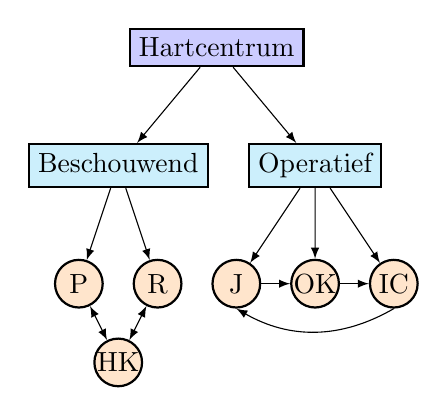
\begin{tikzpicture}[%
                    level 1/.style={sibling distance=2.5cm},
                    level 2/.style={sibling distance=1cm,inner sep=0,minimum size=4ex},
                    ->,
                    hoofd/.style={draw,thick,fill=blue!20},
                    function/.style={draw,thick,fill=cyan!20},
                    afdeling/.style={draw,thick,circle,fill=orange!20}
        ]
    \node[hoofd] {Hartcentrum}
        child { node[function,text depth=depth("p")] {Beschouwend} 
            child { node[afdeling](p) {P} }
            child { node[afdeling] (r) {R} }
        }
        child { node[function] {Operatief} 
            child { node[afdeling] (j) {J} }    
            child { node[afdeling] (ok) {OK} }
            child { node[afdeling] (ic) {IC} }
        }
    ;
\node[yshift=-1cm,afdeling,inner sep=0,minimum size=4ex] (hk) at ($(p)!.5!(r)$) {HK};
\path[<->]
    (hk) edge (p)
    (hk) edge (r);
\path[->]
    (j) edge (ok)
    (ok) edge (ic) 
    (ic.south) edge[bend left] (j.south);
\end{tikzpicture}
\caption{Verdeling van de functies van de verschillende afdelingen van het hartcentrum. De OK en IC worden gedeeld door afdelingen die niet tot het hartcentrum behoren.}
\label{fig:hartcentrum_verdeling}
\end{marginfigure}
\section{Behandelingen \& patiënten}

Op het hartcentrum worden de volgende behandelingen uitgevoerd:

    \begin{itemize}
        \item Thoraxchirurgie
            \begin{itemize}
                \item Kransslagader-bypass (CABG)
            \end{itemize}
        \item Hartkatheterisatie
            \begin{itemize}
                \item Ablatie
                \item Hartklepvervanging
                \item Doteren
                \item Plaatsing Pacemaker of ICD
            \end{itemize}
    \end{itemize}

    Op \afdelingj liggen vooral patiënten die een CABG of een ablatie zijn ondergaan. Deze patiënten zijn vooral van seniore leeftijd. Deze patiënten hebben vaak hypertensie, wat verklaart de verspreiding van anti-hypertensie medicijnen door de verpleging.

    Aan de andere kant liggen op de afdeling~P en afdeling~R patiënten die relatief minder invasieve operaties ondergaan zijn. Deze patiënten liggen derhalve ook minder lang.

    \newthought{De gemiddelde opnameduur} op \afdelingj is één week. Deze week is verdeeld in vier delen: preoperatieve zorg, operatie, intensieve zorg en postoperatieve(zie \cref{fig:tijdspad_opname}). De eerste drie genoemde delen duren twee dagen. 
\begin{marginfigure}
    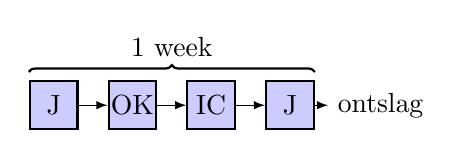
\begin{tikzpicture}[%
                    overstap/.style={draw,thick,fill=blue!20,inner sep=0,minimum size=4ex},
        ]
        \node[overstap] (j) {J};
        \node[right of=j,overstap] (ok) {OK};
        \node[right of=ok,overstap] (ic) {IC};
        \node[right of=ic,overstap] (j1) {J};
        \node[right of=j1,xshift=1ex] (ontslag) {ontslag};
%
        \path[->]
            (j) edge (ok)
            (ok) edge (ic)
            (ic) edge (j1)
            (j1) edge(ontslag) 
            ;
        \draw[decoration={brace,raise=3pt},decorate,thick] (j.north west) -- (j1.north east) node[midway,above,yshift=5pt] {1 week};
    \end{tikzpicture}
    \caption{Tijdspad van opname in hartcentrum \& \afdelingj tot aan ontslag.}
    \label{fig:tijdspad_opname}
\end{marginfigure}
Bij preoperatieve zorg verblijf je één dag op \afdelingj. Op die dag gaat de thoraxchirurg de operatie procedure en voor- en nadelen die hieraan verbonden zijn, toelichten. Verder zal de verpleging enkele praktische zaken bespreken, zoals welke spullen meegenomen moeten geworden en welke spullen thuis moeten blijven.

Na de operatie komt de patiënt terecht op de IC. Hier zijn tijdelijk de intensivisten hoofdbehandelaren.

De IC wordt gevolgd door een overplaatsing naar \afdelingj. Hier worden patiënten weer op de been geholpen. Mijn activiteiten gedurende de zorgstage vonden plaats gedurende deze fase. 
\chapter{Postoperatieve zorg}
Rondom de postoperatieve zorg is een tal aan zorgverleners bij betrokken. De volgende zorgverleners zijn aanwezig op \afdelingj geordend naar positie:
    \begin{enumerate}
        \item Hoofdbehandelaar, de thoraxchirurg\sidenote{De thoraxchirurg is vrijwel afwezig op de afdeling. Hij of zij komt altijd langs voor de operatie en bij ontslag van de patiënt. Zijn primaire taak is een succesvolle operatie uitvoeren.}
        \item Physician assistant \& verpleegkundig specialist
        \item Senior verpleegkundige
        \item Verpleegkundigen
        \item Voedingsassitent, facilitair medewerker \& social worker
    \end{enumerate}

    De physician assistant samen in overleg met de hoofdbehandelaar bepaalt het medisch beleid van alle patiënten op de afdeling. De senior verpleegkundige coördineert de acties van de verpleegkundigen. De voedingsassistent brengt het voedsel rond in de kamers, de facilitair medewerker het was wegbrengen en social worker patiënten opbeuren. Over de werkinhoud wordt later uitgebreid op ingegaan. 

    Verder zijn er de medebehandelaars/consulenten.\sidenote{Een verwant beroepsgroep zijn de hulpbehandelaars. Dit zijn niet-medische specialisten aan wie een gedeelte van de behandeling uitbesteed is. Denk hierbij aan fysiotherapeut. Deze helpt bij de revalidatie en de ademhalingsoefeningen die gewichtig zijn voor het verwijderen van het slijm zonder het scheuren van de wond.} Zij zijn medische specialisten voor de co-morbiditeiten van sommige patiënten. Dit zijn veelvuldig een radioloog, longarts en internist. De radioloog beoordeelt de thoraxfoto, de longarts bepaalt de behandeling, als een afwijking is in de longen, op basis van de beoordeling van de radioloog en de internist komt meestal langs in verband met diabetes.

    \section{Werkinhoud van de verpleging}
De dag van de verpleging begint bij de overdracht. Bij de overdracht worden gegevens over de gezondheidstoestand verandering in de vorige shift van de patiënten verteld aan de verpleegkundigen van de nieuwe shift. 

Na de overdracht wekt de verpleging de patiënten en verdeelt de eerste medicijnen van de dag. De verpleging verdeelt de medicijnen drie maal per dag. De apotheker is verantwoordelijk dat de juiste medicijnen dagelijks beschikbaar is voor elke patiënt op de afdeling.\sidenote{De apotheker stopt dagelijks de medicijnen in de bakjes die zich onder mobiele computer bevinden.} Als de verpleegkundige onbekend is voor de patiënt, dan introduceert hij/zij zichzelf aan de patiënt. 

Verder houdt de verpleegkundige een kleine anamnese door bijvoorbeeld te vragen naar de pijn, stoelgang en gemoedstoestand en sociale \& familiale toestand. Ook behorend tot de anamnese is het meten van het gewicht.

Het lichamelijke verzorging is relatief minder aanwezig op \afdelingj. Vele patiënten kunnen zich redelijk redden in de algemeen dagelijkse levensrichtingen. Dit hangt zeker af welke kamers de verpleegkundige toegedeeld is. De eerste kamers zijn speciaal voor patiënten afkomstig die overgeplaatst worden van IC naar \afdelingj. Deze patiënten vereisen inderdaad meer lichamelijke verzorging.

\newthought{De gegevens verwerkt} de verpleging in het systeem \textit{epic}. Dit systeem standaardiseert en automatiseert de verwerkingen van de observaties.\sidenote{Dit wil zeggen dat de observaties die gemeten kunnen worden al gegeven zijn. Deze observaties zijn verder gecategoriseerd, bijv. bloedwaarden, vitale parameters en gemoedstoestand. Je hoeft alleen de waarde van de observatie te meten.} 

Wanneer de verpleegkundige de gegevens verzameld heeft, rapporteert hij/zij dit bij physician assistant. Dit gebeurt voor de koffiepauze in het zogenaamde ``visitatie''. Met het rapport van verpleegkundige kan de physician assistant het beleid aanpassen. Dus de verpleegkundige is rapporteur en uitvoerder van het medisch beleid, terwijl physician assistant de integrator van de gegevens en determinator van het medisch beleid is(zie \cref{fig:relatie}).
\begin{marginfigure}
    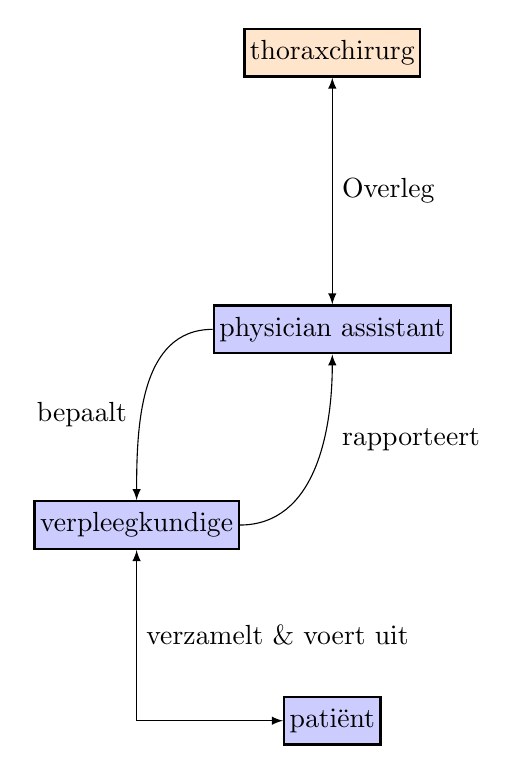
\begin{tikzpicture}[node distance=10em,
                    relatie/.style={draw,thick,fill=blue!20,inner sep=2,minimum size=4ex},
                    boss/.style={draw,thick,fill=orange!20,inner sep=2,minimum size=4ex},
       ]
       \node[relatie] (verpleegkundige) {verpleegkundige};
        \node[relatie,below right of=verpleegkundige] (patient) {patiënt};
        \node[relatie,above right of=verpleegkundige] (physician assistant) {physician assistant};
        \node[above of=physician assistant,boss] (thoraxchirurg) {thoraxchirurg};
        \path[->]
            (physician assistant.west) edge[out=180,in=90] (verpleegkundige) 
            (verpleegkundige) edge[out=0,in=-90] (physician assistant)
            ;
        \draw[<->] (patient) -| (verpleegkundige) node[right,near end] {verzamelt \& voert uit};
        \draw[<->] (thoraxchirurg) -- (physician assistant) node[right,midway] {Overleg};
        \path (verpleegkundige.east)  -| (physician assistant.south)node[right,near end] {rapporteert};
        \path (physician assistant.west)  -| (verpleegkundige.north)node[left,near end] {bepaalt};
    \end{tikzpicture}
    \caption{De relatie tussen verpleegkundige, patiënt en physician assistant. De verpleegkundige voert het medisch beleid van physician assistant en thoraxchirurg uit en verzamelt medische relevante gegevens van de patiënt. Deze gegevens rapporteert de verpleegkundige aan physician assistant.}
    \label{fig:relatie}
\end{marginfigure}
\newthought{Voor het uitvoeren} van het medisch beleid moet de verpleging bekwaam zijn in verpleegtechnische handelingen. De handelingen die het meest op \afdelingj worden verricht, zijn:
    \begin{itemize}
        \item Verwijdering drains
        \item Aanbrengen en verwijdering van veneuze toegangspoorten, zoals PICC
        \item Bloedafname
        \item Verwijdering hechtingen
        \item Wondverzorging
    \end{itemize}

 \newthought{Ten slotte is} het voeren van een ontslaggesprek één van de grootste taken van de verpleging in de postoperatieve fase. Het ontslaggesprek omvat de leefregels voor thuis, de vervolgafspraken op polikliniek, de huisartsenbrief, de medicijnenlijst en de tekens om aan de bel te trekken.
 %%%%%
 \part{Mijn Werkzaamheden \& Reflectie}

 \chapter{Lichamelijk verzorging}
 Zoals eerder vermeld, vindt het wassen relatief in vergelijking tot bijvoorbeeld geriatrie minder vaak op \afdelingj plaats. Men streeft immers tot het behouden van zijn zelfstandigheid\cite{rensen}. Dit wil niet zeggen dat er geen wasbeurten gedurende mijn stageperiode plaats vonden. Mijn eerste mogelijke wasbeurt weigerde ik. Ik vertelde mijn begeleidster dat ik me ongemakkelijk voelde bij het wassen en dat ik bezig zou gaan met het schrijven van mijn logboek. De begeleidster stemde hiermee in. Tijdens het werken aan het logboek vroeg ik de senior verpleegster hoe ik met dit probleem moet aanpakken. Zij antwoordde dat jezelf moet forceren een wasbeurt uit te voeren, als je de ongemakkelijkheid en de angst wilt overwinnen. De volgende dag uitte zich een opportuniteit en die had ik dan ook genomen. Sindsdien gaat het wassen mij goed af.\sidenote{De patiënten die ik tot nu toe gewassen heb, waren weliswaar van hetzelfde sekse.}

Ook heb ik ook een onconventionele wasbeurt uitgevoerd. Met onconventionele wasbeurt duid ik op het verwijderen van lijmresten die zijn ontstaan door de ECG stikkers. Eerst trachtte ik ze te verwijderen met een washandje en lauw water. Dit verliep stroef. Begeleidster vertelde dat je lijmresten niet verwijdert op die manier en reikte me een acetonflesje en pak vol met watjes, wat hielp.

\section{Aankleden}
Betreffend aankleden heb ik alleen geholpen in het aantrekken van elastische kousen en sokken. De eerste keer had ik de binnenkant van de kous niet kunnen bepalen. Als gevolg hiervan trok ik bij de patiënt de kous binnenstebuiten aan. Begeleidster wees erop dat de binnenkant van de kous is de kant waar de antsliplaag zit.

\section{Overige}
Sommige zaken die ik ook uitgevoerd heb maar met minder mate te maken hebben met lichamelijke verzorging zijn toch noemenswaardig. Deze zaken zijn o.a. het verplaatsen van een patiënt in bed, bed opmaken en verschonen, meten van de vitale parameters, het reinigen en aanreiken van instrumenten bij uitvoer van verpleegtechnische handelingen en het brengen van patiënten naar de OK.\sidenote{Bij het brengen naar de OK wordt de patiënt afgezet in de holding. Op de holding worden de laatste checks, waarvan het gewichtigste is het hebben van de juiste patiënt, gemaakt. Na de operatie wordt de patiënt door verpleging opgehaald vanaf de verkoeverruimte.}

\newthought{Gedurend het voeren} van al deze bovengenoemde taken vond het grootste gedeelte van mijn communicatie tussen patiënten plaats. 

\chapter{Communicatie met patiënten}
Het ontwikkelen van een vertrouwen tussen patiënt en arts is één van de gewichtigste voorwaarden van een succesvolle medische consultvoering\cite{veening2009medische}. Aandacht en contact leggen met de patiënt is de eerste stap naar het bepalen van de zorgvraag. Dit verliep redelijk. Ik stelde me voor, mits ik nieuw voor de patiënt was en ze mijn naam niet kenden, en vroeg naar werk, familieopbouw en hobby's. Verkregen deze info begon ik te vragen naar de operatie en het voorafgaande van de operatie.

\newthought{Soms heb ik} het vermoeden dat ik bij sommige patiënten op het grijs gebied van in- en formaliteit zit. Dit speciaal geval bij patiënten waarbij sprake is iets gemeenschappelijk hebben. Dit brengt diepgang in de gesprekken, wat meer dan sufficiënt als bruggenhoofd om uit te vragen naar de zorgvraag.\sidenote{Het voeren van diepgaande gesprekken is de taak van een social worker of gastvrouw/man.}
    Vragend naar raad bij mijn begeleidster antwoordde ze dat een ziekenhuis een sociale vesting is, waarmee bevestigd werd dat ik niet fout bezig was. Echter zei een patiënt dat een verpleegster te zakelijk was. Een verpleegster is een deskundige, wat dan weer impliceert dat ik te informeel ben geweest.

    \newthought{Twee merkwaardige situaties} ervoer ik in een gesprek bij twee verschillende patiënten. Bij één patiënt verweet zijn ellende aan zijn sedatieve levensstijl en adviseerde \textit{mij} om genoeg te bewegen. 

    De andere patiënt barstte uit in tranen gedurende het gesprek. Er was niet alleen niet sprake van tegenspoed bij haarzelf maar ook bij haar naasten. Op dat moment zat ik in dilemma betreft handelen: weglopen, blijven staan of hand op de schouder leggen en zeggen dat alles goed komt. Uiteindelijk besloot ik voor de laatste. Dit leek de juiste keuze, want ze beurde een beetje op.

    \newthought{Communicatieproblemen waren te} danken aan een geen gemeenschappelijke voertaal tussen patiënten en mij. Meeste patiënten spreken Fries dat ik matig beheers. Verder gebruiken de patiënten een eigen jargon voor bepaalde zaken, zoals een hartfilmpje voor ECG en de vredespijp voor de bronchodilator.

\chapter{Waarom de zorg?}
\marginnote{%
\epigraph{%
Alleen in de mate waarin de mens zijn leven zin geeft, verwezenlijkt hij ook zichzelf.
}
{\it Viktor Frankl, Oostenrijkse neuroloog en psychiater (1905-1997)}
}
Een persoon spant zich nimmer in voor een zaak zonder op een bepaalde manier terugbetaald te worden. Deze manier is voor sommige personen geld of eer. In de zorg is zij de dank van de patiënten voor het werken aan het hoogste goed: zieke mensen doen genezen. Het beoogde kan niet door elk lid van team, hetzij een arts hetzij verpleegkundige, afzonderlijk bereikt worden maar alleen bij gezamenlijk inzet. Dit betekent dat elk zorgverlener even relevant is, wat reflecteert in het subtiele onderscheid in de uniformen en de omgang tussen de verschillende zorgverleners. Dankzij de stage weet ik dat de rest van zorgverleners precies dezelfde mentaliteit hebben als ik. 
\printbibliography
\end{document}
